




\section{Info}

\subsection{ADN - liste}
\begin{exercice}[Informatique]
Les questions sont plus ou moins indépendantes. Toutes les fonctions écrites (ou mentionnées) dans les questions précédentes peuvent être utilisées a posteriori. \\


Il est devenu habituel de dire que l'ADN se présente comme un texte composé à l'aide de quatre lettres A,C,G,T, qui s'enchaînent sans interruption et qui est orienté avec un début et une fin. 

%On suppose que l'on a à notre disposition une chaine de caractères, appelée \texttt{ADN}, dont les caractères sont les lettres 'A','C','G' ou 'T'. 

On souhaite faire une étude statistique des lettres présentes dans une séquence d'ADN. 
\begin{enumerate}
\item \begin{enumerate}


\item Ecrire une fonction \texttt{frequence\_A} qui prend en argument une chaine de caractères \texttt{ADN}  et qui retourne la fréquence de la lettre A dans cette chaîne. 

\item On souhaite comparer la fréquence d'apparition de la lettre 'A' entre deux séquences d'ADN. Ecrire une fonction Python \texttt{compare} qui prend en argument deux chaines de caractères \texttt{ADN1}, \texttt{ADN2} et retourne 'elles sont proches' si la fréquence de la lettre A dans \texttt{ADN1} et dans \texttt{ADN2} différe de moins de 0.01. La fonction retournera 'elles ne sont pas proches' dans le cas contraire. \\
\end{enumerate}

On s'intéresse maintenant aux acides aminés, il faut alors regarder les codons qui se lisent par trois (cf le tableau de la dernière page), on doit donc diviser la chaîne de caractères par codon. 

\item
\begin{enumerate}
\item Completer (sur votre copie) la fonction \texttt{liste\_codon}  python qui prend en argument une chaine de caractère \texttt{ADN} et qui  retourne une liste dont les éléments sont les codons de la chaîne. (On supposera que la longueur de la chaine de caractères est bien divisible par 3 sans le vérifier dans la fonction) 
\begin{lstlisting}
def liste_codon(ADN):
    L=[]
    for i in range(0,  ,  ):
        L=L+[ADN[  :  ]]
    return(L)
\end{lstlisting}

Exemple : si \texttt{ADN='GCAGAGTTTTGGTGC'}, la liste retournée sera :
\texttt{['GCA','GAG', 'TTT','TGG','TGC']}.\\
 
 \item On suppose que l'on a  créé une liste \texttt{code\_genetique} qui contient tous les codons possibles. \texttt{code\_genetique=['GCA','GCC', 'GCG', ...., 'TAG', 'TGA']}\\
 
Quelle est la longueur de la liste \texttt{code\_genetique} ? Comment obtenir cette longueur avec une commande Python ? \\

\item On suppose que l'on a une chaine de caractères \texttt{ADN} à notre disposition. 
Ecrire une fonction python \texttt{test} qui vérifie si chaque codons de la liste \texttt{L=liste\_codon(ADN)} est bien un codon du code génétique. \\

\item Compléter (sur votre copie) la fonction \texttt{start} qui prend en argument une liste de codons et qui retourne  l'indice de la première fois où l'on trouve le codon START ('ATG'). Si jamais il n'y en a pas, elle devra retourner un message d'erreur. \\ 
\begin{lstlisting}
def start(L):
    i=0
    while L[i]          :
        if i<len(L)-1:
            
        else:
            return('pas de codon START')
    return(  )
\end{lstlisting}

(Vous pouvez aussi proposer une fonction différente si vous ne comprenez pas la logique de celle-ci, mais attention aux problèmes d'indices.) 

\item Ecrire une fonction \texttt{stop} qui prend en argument une liste de codons et qui retourne  l'indice de la première fois où l'on trouve un codon STOP. Si jamais il n'y en a pas, elle devra retourner un message d'erreur. \\

\item Ecrire une fonction \texttt{proteine} qui prend en argument une liste de codons et  retourne la sous-liste des codons entre   le premier codon START et le premier codon STOP après ce codon START.  (Cette sous-liste contiendra les deux codons START et STOP. On ne  se penchera pas sur le problème d'erreurs, et on supposera que  notre liste contient bien un codon START et un codon STOP dans le bon ordre)   \\
\end{enumerate}






A une séquence d’ADN  correspond une unique séquence d’ARN grâce aux règles de complémentarité : G  et   C sont inversé, A devient U et T devient A. Par exemple, la séquence d’ADN 'AATCGA' est transcrite en 'UUAGCU.' 
\item 
\begin{enumerate}

\item Compléter (sur votre copie)  la fonction python  \texttt{transcription\_lettre} qui prend en argument une lettre correspondant à de l'ADN et qui retourne la lettre d'ARN correspondante. 
\begin{lstlisting}
def transcription_lettre(lettre):
	if lettre==   :
		lettre='G'
	elif          :
		lettre='C'
	elif lettre=='A':
	
	elif          :
		lettre=
    return(       )
\end{lstlisting}

\item Ecrire une fonction python \texttt{transcription} qui prend en argument une chaine de caractères correspondant à de l'ADN et qui retourne la chaine de caractères d'ARN correspondante. 


Parfois il y  a  des erreurs dans la transcription et une lettre est mal transmise. 

\item Ecrire une fonction python \texttt{mutation} qui prend en argument une chaine de caractères (correspondant à de l'ADN) et qui retourne une  chaine de caractères où les lettres 'C' et 'G' sont inversées avec probabilité  99\% et non inversée avec probabilité 1\%, la lettre 'A' est bien changée en 'U' avec probabilité 99\% et changée en 'C' avec probabilité 1\% et la lettre 'T' devient la  lettre 'A' avec proba 99\% et changée en 'U' avec proba 1\%  . Après l'avoir importée, on pourra utiliser la fonction random() qui retourne un réel aléatoire entre 0 et 1. 

\end{enumerate}

\end{enumerate}


\end{exercice}



\begin{figure}[h]
\centering
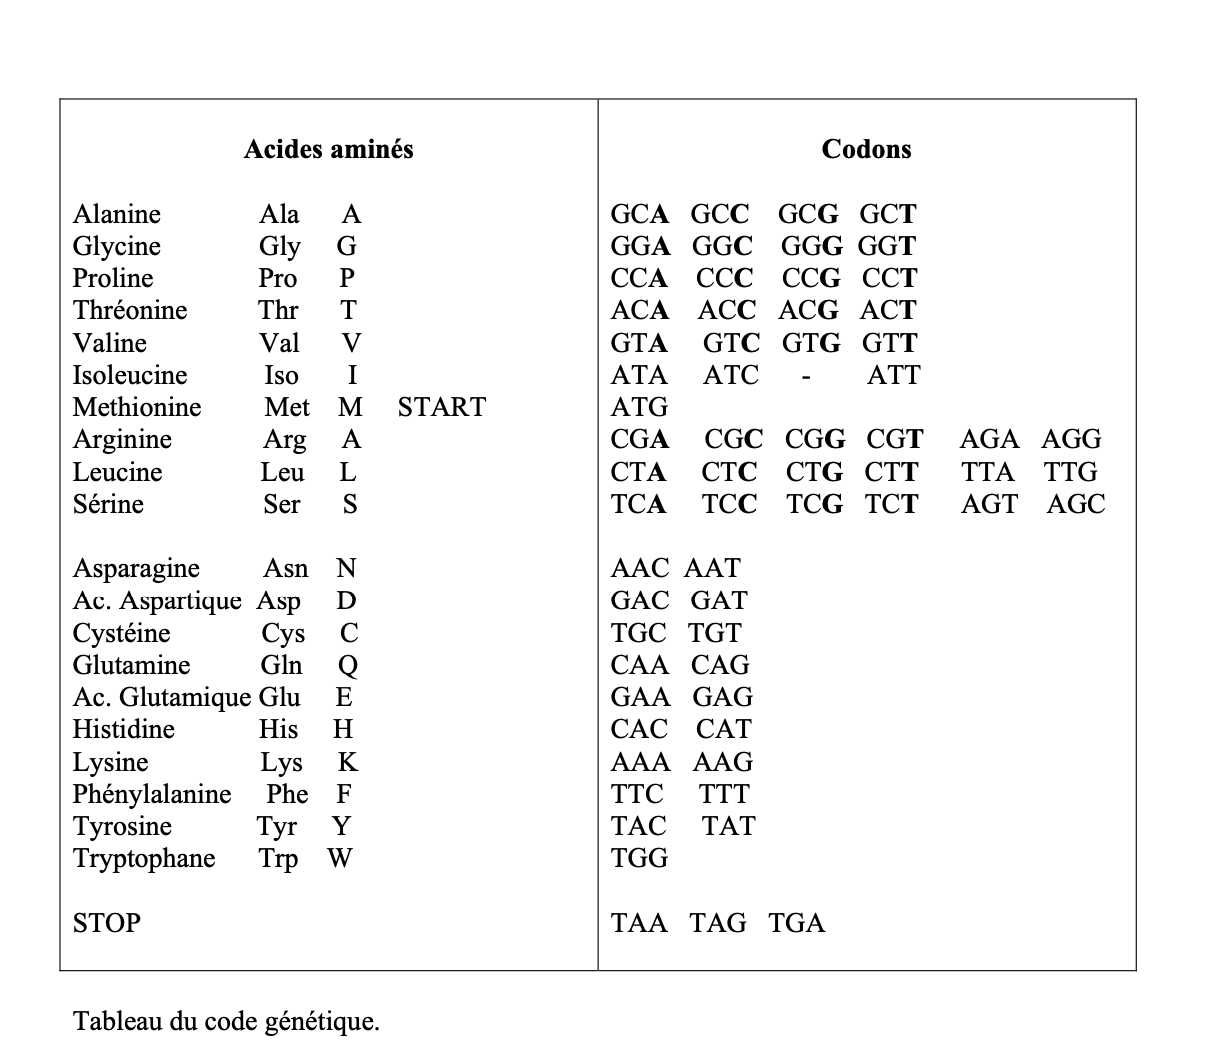
\includegraphics[scale=0.6]{code}
\end{figure}


\begin{correction}

\end{correction}

%--------

\subsection{Lancers de dés. }



\begin{exercice}
Pour toutes les questions d'informatique on pourra utiliser les fonctions créées (ou citées) dans les questions précédentes. 

On considère l'expérience suivante : on effectue une suite de lancers d'un dé  équilibré. On suppose les lancers indépendants. 

Pour tout entier $n$ on note $F_n $ l'événement 
: ' on obtient 6 au  lancer $n$.' 

et $T_n$ l'événément : ' on obtient 6 pour la première fois au lancer $n$'.

\begin{enumerate}
\item Exprimer $T_n$ en fonction des $(F_k)_{k\in \intent{0,n}}$
\item En déduire que $P(T_n) = \frac{5^{n-1} }{6^n}$. 
\item Créer une fonction Python \texttt{premier\_six} qui simule le lancer d'un dé et retourne la première fois où l'on obtient le nombre 6. 
\item Créer une fonction Python \texttt{moyenne\_empirique} qui prend en argument un nombre $N$ représentant le nombre d'itérations de l'expérience et qui retourne la valeur moyenne du nombre de lancers nécessaire pour obtenir le premier 6. 
\item Soit $n\in \N$. On note $B_n$ l'événement 'On obtient  au moins un 6 dans les $n$ premiers lancers'. Exprimer $\overline{B_n}$  en fonction des $(F_k)_{k\in \intent{0,n}}$
\item En déduire $P(B_n)$. 
\item Créer une fonction  Python \texttt{combien\_de\_six} qui prend en argument un nombre $n$ qui correspond au nombre de lancers et retourne le nombre de $6$ obtenu pendant les $n$ lancers. 
%\item Créer une fonction \texttt{frequence\_six} qui prend en argument un nombre   $n$ qui correspond au nombre de lancers et un nombre $N$ qui correspond au nombre d'itérations de l'expérience et qui retourne le nombre moyen de $6$ obtenu au cours des $n$ lancers. 

\item Soit $k\in \N$. On note $C_k$ l'événement 'on obtient $k$ six au cours des 100 premiers lancers'.

 Calculer $P(C_k)$ en fonction de $k$. 
\item Créer une fonction Python \texttt{evenement\_C} qui prend en argument un nombre $k$ et retourne \texttt{True} si on a obtenu exactement $k$ six au cours des 100 premiers lancers et \texttt{False} sinon. 
\item Créer une fonction \texttt{frequence\_C} qui prend en argument un nombre $k$ et un nombre $N$ qui correspond au nombres d'itération de l'expérience et  retourne la fréquence des expériences pour lequel on a obtenue exactement $k$ six pour 100 lancers. 

\end{enumerate}

\end{exercice}


\begin{correction}
\begin{enumerate}
\item $\ddp T_n = \bigcap_{k=1}^{n-1} \overline{F_k}  \cap F_n$
\item $P(F_k) = \frac{1}{6}$  et $P( \overline{F_k}) = \frac{5}{6}$. Les lancers sont indépendants donc 
\begin{align*}
P(T_n) &= \left(\prod_{k=1}^{n-1}  P( \overline{F_k} )\right) P (F_n)\\
&= \left(\prod_{k=1}^{n-1}  \frac{5}{6}\right) \frac{1}{6}\\
&= \frac{5^{n-1}}{6^n}
\end{align*}
\item cf dernière page
\item cf dernière page
\item $\overline{B_n} = \bigcap_{k=1}^{n} \overline{F_k}  \cap F_n$
\item $P(B_n) = 1- P(\overline{B_n} ) = 1- \left(\frac{5}{6}\right)^n$
\item cf dernière page
\item L'univers est la suite des 100 lancers de dés, son cardinal est $6^{100}$ 
Le cardinal de l'événement  est $\binom{100}{k}1^k 5^{100-k}$ (position des dés donnant 6 $\times$ possibilités pour 
 ces dés  , $\times $ posiibilités pour les autres dés)
 On obtient 
 $$P(C_k)  =\frac{\binom{100}{k} 5^{100-k}}{6^{100}}$$

\end{enumerate}
\end{correction}



%------
%---

\subsection{$u_{n+1} = \cos(u_n)$}

\begin{probleme}[Informatique]
Soit $\suiteu$ la suite définie par $\left\{ \begin{array}{ll} 
u_0&=0\\
u_{n+1} &= \cos(u_n)
\end{array}\right.$

\begin{enumerate}
\item Ecrire une fonction \texttt{suite\_u} qui prend comme paramètre d'entrée un entier $n$ et calcule la valeur de $u_n$ correspondante. 
\item On souhaite étudier le comportement de la suite $\suite{u}$, ou tout du moins de ces premiers termes. Ecrire pour cela un programme qui trace un graphique sur lequel se trouvent les points $(n,u_n)$ pour $n\in \intent{0,20}$.

\begin{minipage}[t]{0.4 \textwidth}
On obtient le graphe suivant
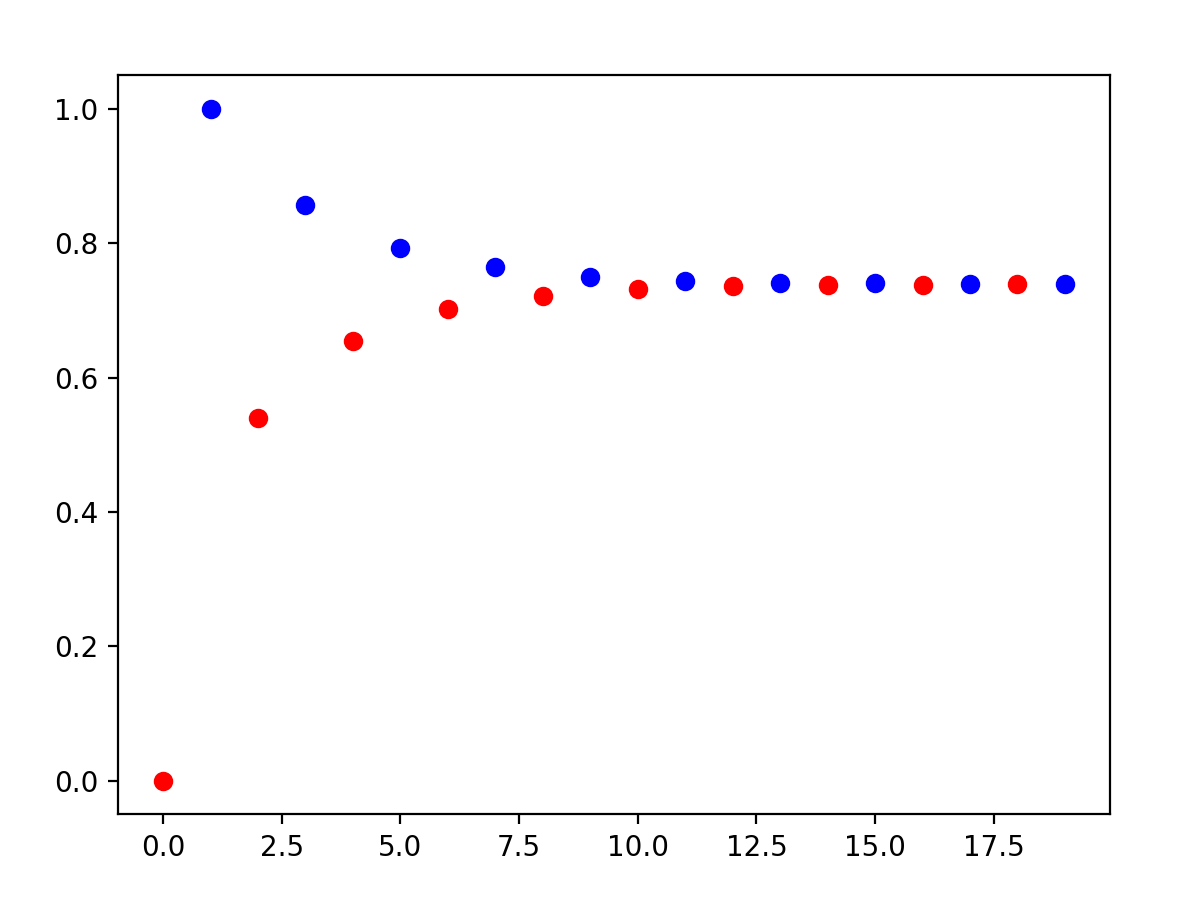
\includegraphics[scale=0.3]{suiteu}

\end{minipage}
\hfill\vline\hfill
\begin{minipage}[t]{0.5 \textwidth}
Les suites $(u_{2n})$ et $(u_{2n+1})$ semblent adjacentes, et converger vers une même limite $\ell$, de sorte que :
$$\lim_{n\tv +\infty} u_n =\ell.$$
En particulier, $\ell$ semble toujours appartenir à l'intervalle d'extrémités $u_n$ et $u_{n+1}$ pour tout entier $n\in \N$, ce qui s'écrit :
$$\forall n\in N, |\ell - u_n| \leq |u_{n+1} - u_n|$$
Nous admettrons tous ces résultats sans démonstration pour la suite. 
\end{minipage}
\item Justifier que le réel $\ell$ satisfait $\ell = \cos(\ell)$ 
\item Proposer un programme permettant de tracer les courbes représentatives des fonctions $f : x\mapsto \cos(x)$ et $g : x \mapsto x$ sur l'intervalle $[0,1]$. \\
Après exécution, ce programme génère le graphe suivant : 
\begin{center}
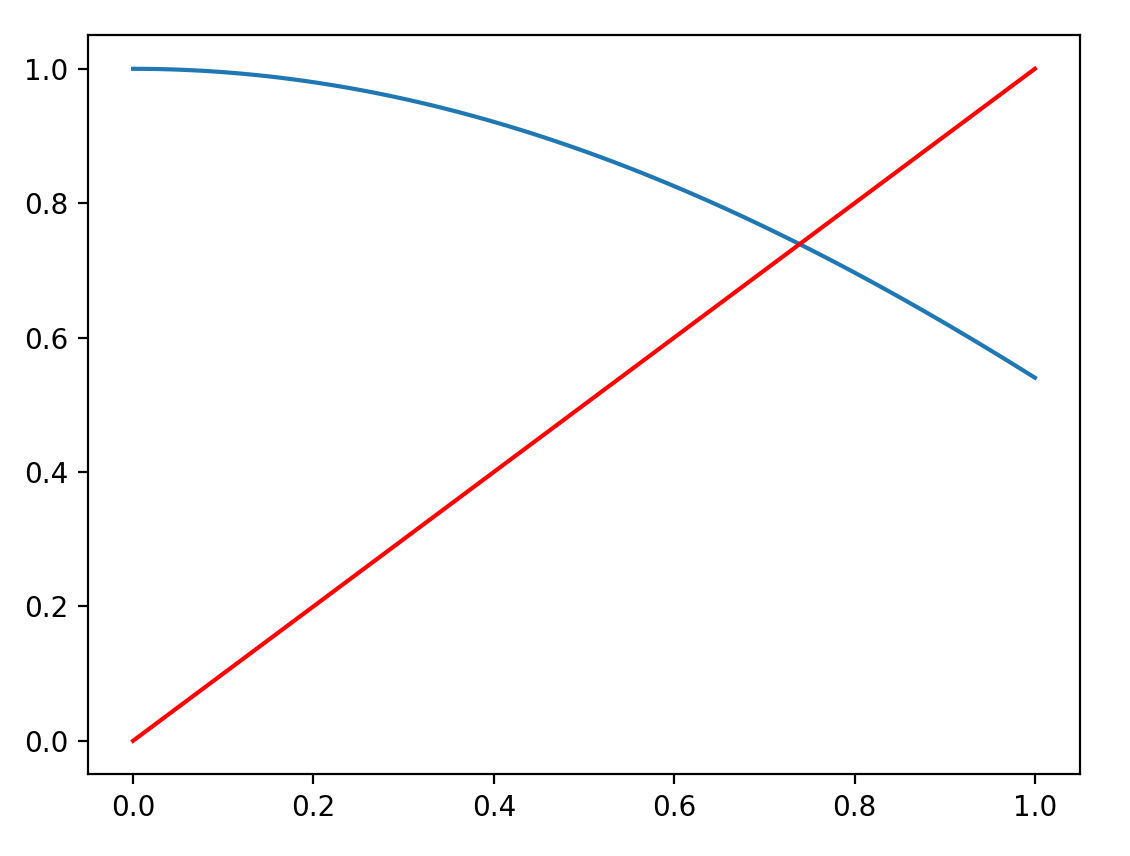
\includegraphics[scale=0.4]{cos}
\end{center}
Déterminer par lecture graphique une valeur approchée de $\ell$. 
\item \begin{enumerate}
\item Ecrire une fonction \texttt{premier\_entier(p)} qui prend comme paramètre d'entrée un entier $p$ et renvoie le plus petit entier tel que $|u_{n+1} - u_n| \leq 10^{-p}$
\item En déduire une fonction $\texttt{approx(p)}$ qui prend comme paramètre d'entrée un entier $p$ et renvoie une valeur approchée de $\ell $ à $\pm 10^{-p}$ prés. 
\end{enumerate}
\item On souhaite déterminer une valeur approchée de $\ell $ par une autre méthode en utilisant un algorithme de dichotomie. On considère pour cela la fonction $h : x \in [0,1] \mapsto x- \cos(x).$
\begin{enumerate}
\item Monter que $h$ s'annule en un unique point de $\alpha \in [0,1]$ et que $\alpha =\ell$. 
\item On suppose avoir défini la fonction $h$ sur Python. Compléter la fonction suivante, qui prend comme paramètre d'entrée un réel $\epsilon>0$ et qui renvoie une valeur approchée de $\ell$ à $\epsilon $ prés à l'aide de la méthode de la dichotomie. 
\begin{lstlisting}
def dichotomie(epsilon):
    a=0
    b=1

    while      >    :
        milieu = (a+b)/2
        if h(milieu)*h(a)<0:
            
        else:
            
    return(a)
\end{lstlisting}


\end{enumerate}
\end{enumerate}




\end{probleme}

\begin{correction}
3 - Comme $u_n$ converge vers $\ell$ par unicité de la limite $u_{n+1}$ converge vers $\ell$. Comme $\cos$ est continue sur $\R$ on a 
$lim_{n\tv\infty} \cos(u_n) = \cos(\ell)$. Ainsi $\ell =\cos(\ell)$\\
4- $\ell \simeq 0.8$\\
6-a C'est une application du théorème de la bijection. 
$h$ est continue et dérivable sur $[0,1]$ et $h'(x) = 1+sin(x) >0$ donc $h$ est strictement croissante. $h(0)=-1$ et $h(1)= 1-\cos(1)>0 $ donc d'après le théorème de la bijection il existe un unique $\alpha \in [0,1]$ tel que $h(\alpha) =0$. 
$\alpha$ vérifie donc $\alpha-\cos(\alpha)=0$ cad $\alpha =\cos(\alpha)$ par unicité de la solution sur l'intervalle $[0,1]$ il est égale à $\ell$. 

\end{correction}


%%%%

\subsection{Mandelbrot}

\begin{exercice}[Ensemble de Mandelbrot]
Soit $\suite{z}$ la suite définie par $z_0=0$ et 
$$z_{n+1} =z_n^2 +c$$
où $c\in \bC$ est un complexe. 

Selon la valeur de $c$, il y a deux possibilités : soit $\suite{z}$ reste bornée, soit son module tends vers l'infini. Le but de ce problème est d'écrire un algorithme qui permet de tracer l'ensemble des $c$ pour lesquels la suite $\suite{z}$ reste bornée. Cette ensemble s'appelle l'ensemble de Mandelbrot. 
\begin{enumerate}
\item Que vaut la suite $\suite{z}$ pour $c=0$. Est ce que $c=0$ appartient à l'ensemble de Mandelbrot ?

\item Que valent les premières valeurs ($n=0,1,2,3,4$) de la suite $\suite{z}$ pour $c=i$.  A votre avis est-ce-que $c=i$ appartient à l'ensemble de Mandelbrot ? 
\item Même question pour $c=1+i$ (pour $n=0,1,2,3$).
\item Ecrire une fonction Python \texttt{suite\_z} qui prend en argument un entier $n\in \N$ et un complexe $c\in \bC$ et qui retourne la valeur de $z_n$.
\item On peut montrer que $c$ appartient à l'ensemble de Mandelbrot si et seulement pour tout $n\in \N$,  $|z_n|<2$.
On suppose pour simplifier qu'un nombre $c$ appartient à l'ensemble des Mandelbrot si et seulement si  pour tout $n\in \intent{0,100},   \, |z_n|<2$.
Ecrire une fonction \text{verif} qui prend un nombre complexe $c$ et retourne \texttt{True} si $c$ appartient à l'ensemble de Mandelbrot et \texttt{False} sinon. 
\item Ecrire une fonction \texttt{tracer} qui prend en argument deux réels $(x,y)$ et qui trace le point $(x,y)$ sur un graphique si le point d'affixe $x+iy$ appartient à l'ensemble de Mandelbrot. 
\item Ecrire un script python qui teste  si les points de coordonnées $\left( \frac{i}{100}, \frac{j}{100}\right)$ pour $i, j\in \intent{-100,100}$ appartiennent à l'ensemble de Mandelbrot et les trace le cas échéant. 
\end{enumerate}
\begin{center}
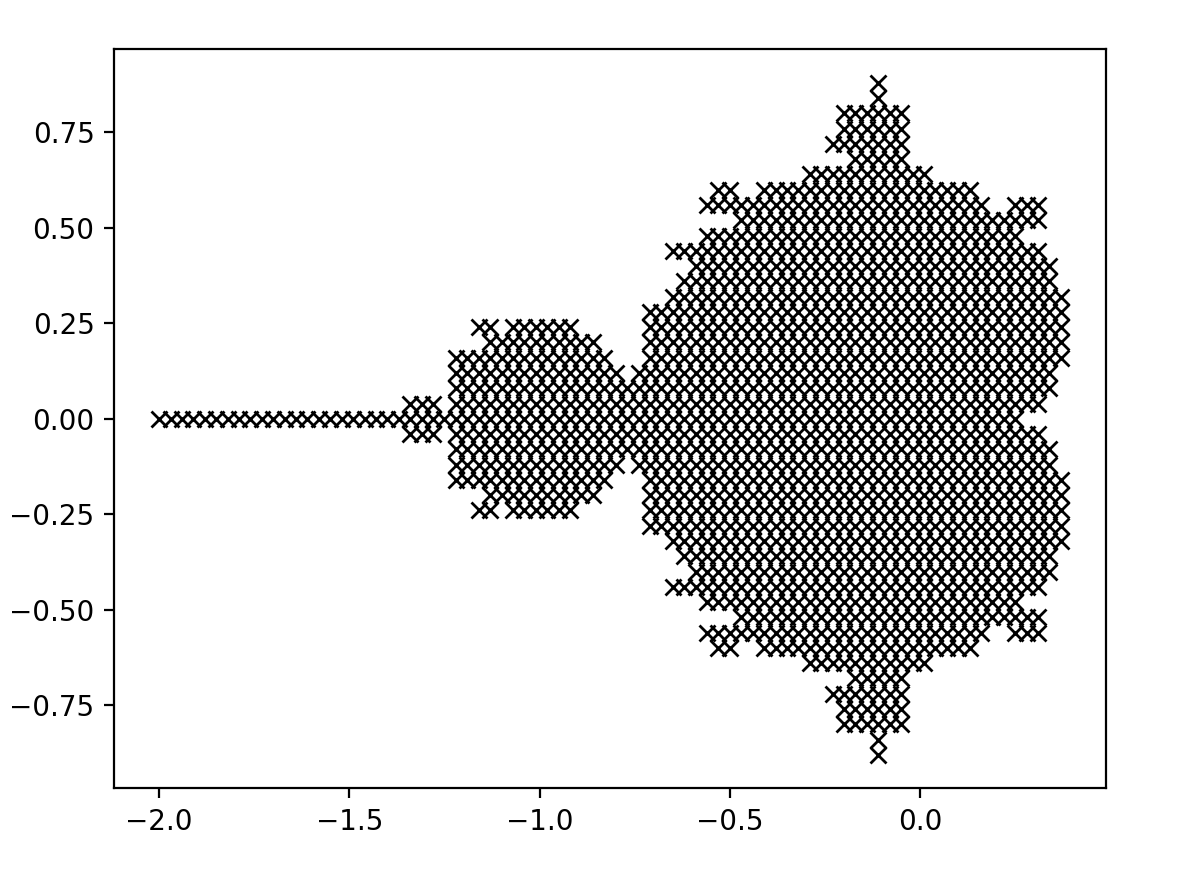
\includegraphics[scale=0.4]{mandelbrot.png}
\end{center}

\end{exercice}


\begin{correction}
\begin{enumerate}
\item Pour $c=0$ la suite $\suite{z}$ est constante égale à $0$. $0$ appartient donc à l'ensemble de Mandelbrot. 
\item Pour $c=i$, $z_0=0$, $z_1=i$, $z_2= i^2+i=-1+i$, $z_3= (-1+i)^2 +i = -i$, $z_4=(-i)^2+i = -1+i$. La suite semble périodique et donc le module est borné. Ainsi $c=i$  appartient donc à l'ensemble de Mandelbrot. 

\item Pour $c=1+i$ : $z_0=0$, $z_1=1+i$, $z_2=(1+i)^2+1+i=1+3i$, $z_3= (1+3i)^2 +1+i = -7+7i$, $z_4=(-7+7i)^2+1+i= 49(-1+i)^2+1+i = 49(-2i) +1+i = 1-97i$. Le module semble tendre vers l'infini. 
$c=1+i$ n'appartient donc pas à l'ensemble de Mandelbrot. 


\end{enumerate}
\begin{lstlisting}[language=Python]
def suite_z(n,c):
    z=0
    for i  in range(n):
        z=z**2+c
    return(z)

def verif(c):
    for n in range(101):
        if suite_z(n,c)>2:
            return(False)
    return(True)

import matplotlib.pyplot as plt
def tracer(x,y):
    c=x+y*1j
    if verif(c)==True:
        plt.plot(x,y,'kx')

for x in range(-100,101):
    for y in range(-100,101):
        tracer(x/100,y/100)
plt.show()

\end{lstlisting}

\end{correction}


%%%%
\subsection{Pendu}

\begin{exercice}


\begin{enumerate}
\item On suppose que l'on dipose d'une liste \texttt{dictionnaire} contenant tous les mots du dictionnaire. (Pour vos testes, créer une liste  \texttt{dictionnaire} contenant trois mots : 'coucou', 'olivier', 'matrice' )

Ecrire une fonction \texttt{mots\_de7lettres} qui retourne une liste ne contenant que les mots de 7 lettres du \texttt{dictionnaire}.

\item Ecrire une fonction \texttt{choix\_mot}, qui choisit un mot de 7 lettres aléatoirement.
(On pourra utiliser la fonction \texttt{len} qui prend en argument une chaine de caractères et qui retourne sa taille, (comme pour les listes) ) 

\item Ecrire une fonction \texttt{transform} qui prend en argument une chaine de caractères \texttt{S} et retourne une liste dont chaque entrée est une lettre de la chaine \texttt{S}.

\item Créer une fonction \texttt{test\_lettre} qui prend en argument un mot \texttt{M} et une lettre \texttt{a} et retourne la (ou les) position de la lettre \texttt{a} dans le mot \texttt{M}. Si \texttt{a} n'est pas dans le mot, la fonction retournera la liste vide. 

Exemples : \texttt{test\_lettre}('olivier', 'i') --> [2, 4] et \texttt{test\_lettre}('olivier', 'w') --> []

\item Ecrire une fonction  \texttt{reponse} qui prend en argument deux chaines de caractères. L'une \texttt{M} correspondant au mot que l'on doit trouver et l'autre \texttt{P} correspondant à la proposition du joueur. Si le joueur propose une seule lettre alors  la fonction \texttt{reponse}  retourne la (ou les places) de la lettre dans le mot \texttt{M}, si le joueur propose un mot (donc plusieurs lettres) alors la fonction \texttt{reponse} retourne \texttt{True} si le mot est bon et une liste vide si le mot est mauvais. (La liste vide permet d'être dans le même cas que si on avait donné juste une lettre qui n'est pas dans le mot) 

\item Ecrire une fonction \texttt{lettre\_connue} qui prend en argument un mot \texttt{M}  (correspondant au mot à trouver) et une liste \texttt{L}  (qui correspond au position des lettres déjà trouvées) et qui retourne une chaine de caractères où les lettres dont la position sont dans \texttt{L} s'affiche en claire et sinon sont remplacées par des '*'

Exemple : \texttt{lettre\_connue} ('olivier', [1,2,5]) retourne '*li**i**' 
\texttt{lettre\_connue} ('matrice', [0,1,2]) affiche 'ma*****'
 

 \item Compléter le code suivant qui permet de jouer au jeu du pendu  sans limite d'essais. 
\newpage
 \begin{lstlisting}
 def pendu():
    mot_a_trouver=.....
    mot_propose=''
    list_lettres_connues=[]
    while mot_propose != ......:    
        l=lettres_connues(.... , ....)
        # On affiche les lettres deja trouvees par le joueur)
        print(l)

        mot_propose = input('Donner une lettre ou une proposition') 
        #on demande au joueur une nouvelle lettre ou une nouvelle propostion

        rep=reponse(...., .... ) 
        #on analyse la reponse.

        if ...==.... : #si le joueur a trouve le bon mot
            print( ....  )# on le felicite
            return #on arrete le programme

        else: #sinon
            if len(rep)......:  #soit le mot n'est pas le bon ou la lettre n'est pas dans le mot
                print('essaye encore') #et on lui dit de reesayer

            else:
                print('il y a ' +...... +' lettre ' + .... )  
                #on affiche le nombre de fois ou la lettre proposee 
                #apparait dans le mot cherche
                
                list_lettres_connues=....+.... 
                #et on ajoute a la liste des lettres 
                #connues les nouvelles lettres.

 \end{lstlisting}
 
 \item Améliorer la fonction \texttt{pendu} pour que le programme s'arrête après 10 essais infructueux et affiche à chaque essais le nombre de tentatives restantes. 


\end{enumerate}
\end{exercice}
\begin{correction}

\end{correction}


\subsection{Pivot de Gauss}



\begin{exercice} [Extrait du Concours Agro-Veto 2019]
Des éléments de syntaxe Python, et en particulier l'usage du module numpy, sont donnés en annexe . Dans tout ce qui suit, les variables $n, p, A, M, i, j$ et $c$ vérifient les conditions suivantes qui ne seront pas rappelées à chaque question :
\begin{itemize}


\item $n$ et $p$ sont des entiers naturels tels que $p \geq n \geq 2$;
\item $A$ est une matrice carrée à $n$ lignes inversible;
\item $M$ est une matrice à $n$ lignes et $p$ colonnes telle que la sous-matrice carrée constituée des $n$ premières colonnes de $M$ est inversible;
\item  $i$ et $j$ sont des entiers tels que $0 \leq i \leq n-1$ et $0 \leq j \leq n-1$;
\item  $c$ est un réel non nul.
\end{itemize}
On note $L_{i} \leftarrow L_{i}+c L_{j}$ l'opération qui ajoute à la ligne $i$ d'une matrice la ligne $j$ multipliée par c.
\begin{enumerate}


\item Soit la fonction initialisation:
\begin{lstlisting}{python}
def initialisation(A):
    n = np.shape(A)[0]
    mat = np.zeros((n,2*n))
    for i in range(0, n):
        for j in range(0, n):
            mat[i,j] = A[i,j]
    return(mat)
\end{lstlisting}
Pour chacune des affirmations suivantes, indiquer si elle est vraie ou fausse, en justifiant. L'appel initialisation (A) renvoie:
\begin{enumerate}


\item une matrice rectangulaire à $n$ lignes et $2 n$ colonnes remplie de zéros;
\item une matrice de même taille que $A$;
\item une erreur au niveau d'un range;
\item une matrice rectangulaire telle que les $n$ premières colonnes correspondent aux $n$ colonnes de $A$, et les autres colonnes sont nulles.\end{enumerate}
\item  Les trois fonctions multip, ajout et permut suivantes ne renvoient rien : elles modifient les matrices auxquelles elles s'appliquent.
\begin{enumerate}


\item Que réalise la fonction multip?
\begin{lstlisting}{python}
def multip(M, i, c):
    p = np.shape(M)[1]
    for k in range(0, p):
        M[i,k] = c*M[i,k]
\end{lstlisting}


\item Compléter la fonction ajout, afin qu'elle effectue l'opération $L_{i} \leftarrow L_{i}+c L_{j}$.
\begin{lstlisting}{python}
def ajout(M, i, j, c):
    p = np.shape(M)[1]
    for k in range(0, p):
        _____ ligne(s) a completer _____ 
\end{lstlisting}

\item Écrire une fonction permut prenant pour argument $M, i$ et $j$, et qui modifie $M$ en échangeant les valeurs des lignes $i$ et $j$.
\end{enumerate}
Dans la suite du sujet, l'expression "opération élémentaire sur les lignes" fera référence à l'utilisation de permut, multip ou ajout.
\item  Soit la colonne numéro $j$ dans la matrice $M$. On cherche le numéro $r$ d'une ligne où est situé le plus grand coefficient (en valeur absolue) de cette colonne parmi les lignes $j$ à $n-1$. Autrement dit, $r$ vérifie :
$$
|A[r, j]|=\max \{|A[i, j]| \text { pour } i \text { tel que } j \leq i \leq n-1\} .
$$
Écrire une fonction \texttt{rang\_pivot} prenant pour argument $M$ et $j$, et qui renvoie cette valeur de $r$.

 Lorsqu'il y a plusieurs réponses possibles pour $r$, dire (avec justification) si l'algorithme renvoie le plus petit $r$, le plus grand $r$ ou un autre choix.
 
  (L'utilisation d'une commande max déjà programmée dans Python est bien sûr proscrite.)
  
\item Soit la fonction mystere:
\begin{lstlisting}{python}
def mystere(M):
    n = np.shape(M)[0]
    for j in range(0, n):
        r = rang_pivot(M, j)
        permut(M, r, j)
        for k in range(j+1, n):
            ajout(M, k, j, -M[k,j]/M[j,j])
        print(M) 
\end{lstlisting} 

\begin{enumerate}
\item On considère dans cette question l'algorithme mystere appliqué à la matrice \[M_{1}=\left(\begin{array}{ccc}3 & 2 & 2 \\ -6 & 0 & 12 \\ 1 & 1 & -3\end{array}\right)\] Indiquer combien de fois la ligne print (M) est exécutée ainsi que les différentes valeurs qu'elle affiche
\item De façon générale, que réalise cet algorithme?
\end{enumerate} 
\item On considère la fonction reduire:
\begin{lstlisting}{python}
def reduire(M):
    n = np.shape(M)[0]
    mystere(M)
    for i in range(0, n):
        multip(M, i, 1/M[i,i])
    #Les lignes suivantes sont \'a compl\'eter :
        __________________________        
\end{lstlisting}
Compléter la fonction afin que la portion de code manquante effectue les opérations élémentaires suivantes sur les lignes :

pour $j$ prenant les valeurs $n-1, n-2, \ldots, 1$, faire :


\hspace{2cm}	pour $k$ prenant les valeurs $j-1, j-2, \ldots, 0$, faire :

$$
\mathrm{L}_{\mathrm{k}} \leftarrow \mathrm{L}_{\mathrm{k}}-\mathrm{M}[\mathrm{k}, \mathrm{j}] \mathrm{L}_{\mathrm{j}}
$$



Indiquer ce que réalise cette fonction.
\end{enumerate}

\begin{center}
\textbf{\huge{Annexe}}
\end{center}
On considère que le module numpy, permettant de manipuler des tableaux à deux dimensions, est importé via import numpy as np. Pour une matrice $M$ à $n$ lignes et $p$ colonnes, les indices vont de 0 à $n-1$ pour les lignes et de 0 à $p-1$ pour les colonnes.

\begin{center}
\begin{tabular}{ll}
\hline \multicolumn{1}{c}{ Python } & \multicolumn{1}{c}{ Interprétation } \\
\hline $\mathrm{abs}(\mathrm{x})$ & Valeur absolue du nombre $x$ \\
\hline $\mathrm{M}[\mathrm{i}, \mathrm{j}]$ & Coefficient d'indice $(i, j)$ de la matrice $M$ \\
\hline $\mathrm{np} \cdot$ zeros $((\mathrm{n}, \mathrm{p}))$ & Matrice à $n$ lignes et $p$ colonnes remplie de zéros \\
\hline $\mathrm{T}=\mathrm{np} . \mathrm{shape}(\mathrm{M})$ & Dimensions de la matrice $M$ \\
$\mathrm{~T}[0]$ ou np.shape $(\mathrm{M})[0]$ & Nombre de lignes \\
$\mathrm{T}[1]$ ou np.shape $(\mathrm{M})[1]$ & Nombre de colonnes \\
\hline $\mathrm{M}[\mathrm{a}: \mathrm{b}, \mathrm{c}: \mathrm{d}]$ & Matrice extraite de $M$ constituée des lignes $a$ à $b-1$ et des \\
& colonnes $c$ à $d-1:$ \\
& si $a$ (resp. $c)$ n'est pas précisé, l'extraction commence à la \\
& première ligne (resp. colonne) \\
& si $b$ (resp. $d)$ n'est pas précisé, l'extraction finit à la dernière \\
& ligne (resp. colonne) incluse \\
\hline
\end{tabular}
\end{center}
\end{exercice}


\begin{correction}

\end{correction}
